%% -*- coding:utf-8 -*-
\documentclass[10pt,pdf,hyperref={unicode}]{beamer}
\input ./preamble.tex
\usetheme{Warsaw}
\title[Cryptography and quantum computations]{Classical
  cryptography\\Quantum computations}
\author{Ivan Murashko}
%\institute{Санкт Петербургский Государственный Политехнический Университет}
\date{}
\begin{document}

\begin{frame}
\titlepage
\end{frame}


\section{Introduction}

\begin{frame}{Introduction}
\begin{itemize}
\item Quantum mechanics
\item Quantum computations
\item Symmetric cryptography. Grover search algorithm (GSA)
\item Public-key cryptography cryptography (RSA, Diffie-Hellman, Elliptic
curve) and Shor's algrorithm.
\end{itemize}
\end{frame}

\section{Quantum mechanics}

\begin{frame}{Quantum world vs Classical one}
   \begin{figure} 
   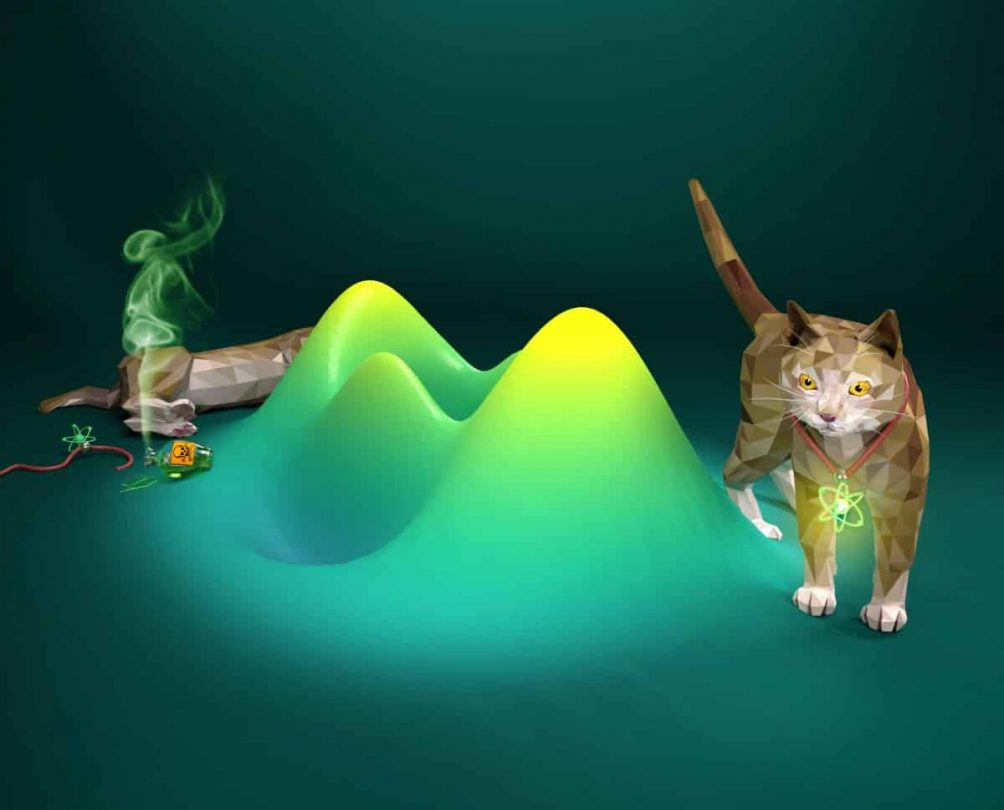
\includegraphics[width=50mm,scale=0.5]{quantumworld.jpg}
  \end{figure}
  They differ. There are 2 examples
  \begin{enumerate}
  \item Schrödinger's cat, two-level atom and q-bit (quantum bit)
  \item Bell experiment, negative probability and quantum logic  
  \end{enumerate}
\end{frame}

\begin{frame}{Two-level atom, q-bit}
\begin{figure}
\centering

\input ../add/quant/picmeasurex.tex

\caption{Energy measurement for two-level atom. The atom is in pure
  state:  $\left|\psi\right> = 
  \frac{1}{\sqrt{2}}\left|a\right> + \frac{1}{\sqrt{2}}\left|b\right>$.
  Device can get either $E_a$ or $E_b$.
}
\label{fig:add:mesure_ex}
\end{figure}
\end{frame}

\begin{frame}{Two-level atom. $E_a$ measurement}
\begin{figure}
\centering

\input ../add/quant/picmeasurex_a.tex

\caption{Energy measurement for two-level atom. The atom is in pure
  state: $\left|\psi\right> = 
  \frac{1}{\sqrt{2}}\left|a\right> + \frac{1}{\sqrt{2}}\left|b\right>$.
  Device got $E_a$. The following wave function collapse occurs as a
  result of the measurement $\left|\psi\right> \to \left|a\right>$
}
\label{fig:add:mesure_ex_a}
\end{figure}
\end{frame}

\begin{frame}{Two-level atom. $E_b$ measurement}
\begin{figure}
\centering

\input ../add/quant/picmeasurex_b.tex

\caption{Energy measurement for two-level atom. The atom is in pure
  state: $\left|\psi\right> = 
\frac{1}{\sqrt{2}}\left|a\right> + \frac{1}{\sqrt{2}}\left|b\right>$.
Device got $E_b$. The following wave function collapse occurs as a
  result of the measurement $\left|\psi\right> \to \left|b\right>$
}
\label{fig:add:mesure_ex_b}
\end{figure}
\end{frame}

\begin{frame}{Schrödinger's cat}
 \begin{figure} 
   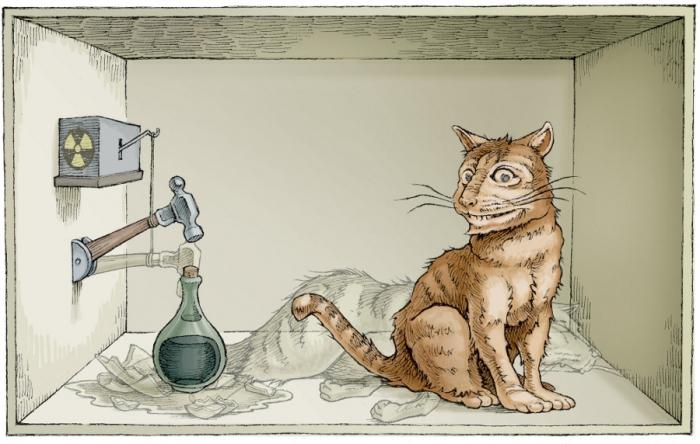
\includegraphics[width=100mm,scale=0.5]{catshred.jpg}
  \end{figure}
\end{frame}

\begin{frame}{Classical bit vs quantum q-bit}
  Classical bit is either $0$ or $1$.

  Quantum q-bit is another case. It's a state
  $\ket{q} = \alpha \ket{0} + \beta \ket{1}$. I.e. as Schrödinger's
  cat it can be $1$ (die) and $0$ (alive) simultaneously
\end{frame}


\begin{frame}{Bell experiment. Classical case}
\[
f = \frac{1}{2}\left(
a b + a' b + a b' - a' b'
\right), a,a',b,b' \in \{-1, +1\}.
\]
therefore
\(
f \in \{-1, +1\}
\)
and
\(
\left|\left<f\right>\right| \le 1
\)
\end{frame}

\begin{frame}{Bell experiment. Quantum case}
\[
\left|\left<f\right>\right| = \sqrt{2} > 1
\]
\end{frame}


\begin{frame}{Negative probabilities}
\[
\left<f\right> = \sum_{a,a',b,b'} p(a,a',b,b') f(a,a',b,b').
\]
therefore for $\left|\left<f\right>\right| > 1$ necessary to have
\[
\exists a,a',b,b': p(a,a',b,b') < 0
\]
\end{frame}

\begin{frame}{Heisenberg inequality}
  \[
  \Delta p \Delta q \ge \frac{\hbar}{2}
  \]
\end{frame}

\begin{frame}{Quantum logic}
  Distributive law is failed for quantum logic:
  \begin{itemize}
  \item $P \land (Q_1 \lor Q_2)$ can be true
  \item but both $P \land Q_1$ as well as $P \land Q_2$ are false
  \end{itemize}
  in other words
  \[
  P \land (Q_1 \lor Q_2) \ne (P \land Q_1) \lor (P \land Q_2)
  \]
  where $\land$ is ``logical and'', $\lor$ is ``logical or''
\end{frame}

\begin{frame}{Quantum logic}
\begin{figure}[H]
  \centering
  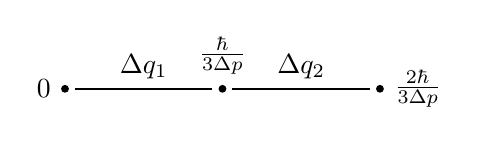
\begin{tikzpicture}[ele/.style={fill=black,circle,minimum
          width=.8pt,inner sep=1pt}]
      \node[ele,label=left:$0$] (a) at (0,0) {};
      \node[ele,label=above:$\frac{\hbar}{3 \Delta p}$] (b) at (2,0) {};
      \node[ele,label=right:$\frac{2 \hbar}{3 \Delta p}$] (c) at (4,0) {};
      \draw[-,thick,shorten <=2pt,shorten >=2pt] (a) to node[above]
           {$\Delta q_1$} (b);
      \draw[-,thick,shorten <=2pt,shorten >=2pt] (b) to node[above]
           {$\Delta q_2$} (c);  
  \end{tikzpicture}
  \caption{Heisenberg inequality. The event $P$ is that momentum has
    uncertainty $\Delta p$ Event $P \land Q_1$ is that particle's
    position is between $0$ and $\frac{\hbar}{3 \Delta p}$. Event
    $P \land Q_2$ is that particle's
    position is between $\frac{\hbar}{3 \Delta p}$ and
    $\frac{2\hbar}{3 \Delta p}$. Particle's position for event $P
    \land Q = (P \land Q_1)
    \lor (P \land Q_2)$ is between $0$ and $\frac{2\hbar}{3 \Delta p}$. The
    events $P \land Q_1$ and $P \land Q_2$ are forbidden by the Heisenberg
    inequality. From other side the event $P \land Q = (P \land Q_1)
    \lor (P \land Q_2)$ is possible}   
\end{figure}
\end{frame}

\section{Quantum computations}

\begin{frame}{Classical computation}
\begin{figure}
\centering

\input ../part4/quantcomp/picclasscomp.tex

\caption{Classical computation. Input has a number $x$ that consists
  of  $n$ bits. Output $y = f\left(x\right)$ is the result that
  consists of $m$ bits}
\label{figQuantCompClassComp}
\end{figure}
\end{frame}

\begin{frame}{Quantum computations}
\begin{figure}
\centering

\scalebox{.8}{\input{../part4/quantcomp/picquantcomp.tex}}

\caption{Quantum computations should be reversible. We have a number
  $x$ as input. The number consists of $n$ q-bits. We also require to
  have a seed of $0$ states ($m$ q-bits). Output also have two parts: the result $\left|y\right> =
  \left|f\left(x\right)\right>$ is described by $m$ q-bits and initial
  state $\left|x\right>$ ($n$ q-bits)} 
\label{figQuantCompQuantComp}
\end{figure}
\end{frame}


\begin{frame}{Quantum computations}
Classical case
\[
x \to f(x)
\]
Quantum case
\begin{eqnarray}
\left|0\right>\left|0\right> + \left|1\right>\left|0\right> + \left|2\right>\left|0\right> +
\dots + \left|x\right>\left|0\right> + \dots \to
\nonumber \\
\to 
\left|0\right>\left|f(0)\right> + \left|1\right>\left|f(1)\right> + \left|2\right>\left|f(2)\right> +
\dots + \left|x\right>\left|f(x)\right> + \dots
\nonumber
\end{eqnarray}
\end{frame}


\section{Grover search algorithm}
\begin{frame}{Needle in a haystack task}
\begin{figure}
\centering

\input ../part4/quantcomp/picsearch.tex

\caption{Search in unstructured data array (search "a needle in a
  haystack"). Classical complexity is $O(N)$}
\label{figQuantCompSearch}
\end{figure}
\end{frame}

\begin{frame}{Grover search algorithm. Scheme}
\begin{figure}
\centering

\scalebox{1.0}{\input{../part4/quantcomp/picgrover.tex}}

\caption{Grover search algorithm. Complexity is $ O(\sqrt{N})$}
\label{figQuantCompGrover}
\end{figure}
\end{frame}

\begin{frame}{Grover search algorithm. Repeating element scheme}
\begin{figure}
\centering

\scalebox{1.0}{\input{../part4/quantcomp/picgroverbase.tex}}

\caption{Grover search algorithm. Grover iteration}
\label{figQuantCompGrover}
\end{figure}
\end{frame}


\begin{frame}{Grover search algorithm. Main principle}
\begin{figure}
\centering

\scalebox{.9}{\input{../part4/quantcomp/picgroverinv.tex}}

\caption{Grover search algorithm. Phase inversion aka conditional inversion}
\label{figQuantCompGroverInv}
\end{figure}
\end{frame}

\begin{frame}{Grover search algorithm. Main principle}
\begin{figure}
\centering

\scalebox{.8}{\input{../part4/quantcomp/picgroverinvmiddle.tex}}

\caption{Grover search algorithm. Grover diffusion operator}
\label{figQuantCompGroverInvMiddle}
\end{figure}

\end{frame}


\begin{frame}{Impact on classical cryptography}
  $O(N) \rightarrow O(\sqrt{N})$
  leads to the following recommendation 
  $AES_{128} \rightarrow AES_{256}$
\end{frame}


\section{Shor's algorithm}
\begin{frame}{Public key cryptography}
\begin{itemize}
\item RSA and factorisation problem 
\item Diffie-Hellman and discrete logarithm
\item Elliptic curve and discrete logarithm
\end{itemize}
\end{frame}

\begin{frame}{RSA and period-finding problem}
\[
N = p \cdot q
\]
\[
f\left(x, a\right) = a^x \mod N.
\]
The period of the function is $T = 2r$, i.e.
\begin{eqnarray}
a^{x+2r} \mod N = a^x \mod N,
\nonumber \\
a^{2r} \equiv 1 \mod N,
\nonumber \\
(a^r + 1)(a^r - 1)  \equiv 0 \mod N
\nonumber
\end{eqnarray}
\end{frame}

\begin{frame}{Shor's algorithm}
\begin{figure}
\centering

\scalebox{.8}{\input{../part4/quantcomp/picquantperiodfinding.tex}}

\caption{ Period finding problem and quantum Fourier's transform}
\end{figure}
\end{frame}


\begin{frame}{Shor's algorithm. Period funding problem for 
  $f\left(x, a\right) = a^x \mod{N}$}
\begin{figure}
\centering

\scalebox{.65}{\input{../part4/quantcomp/picshorquantfourier1.tex}}

\caption{Shor's algorithm. Period funding problem for 
  $f\left(x, a\right) = a^x \mod{N}$, $a=2$, $N = 21$.}
\end{figure}
\end{frame}

\begin{frame}{Shor's algorithm. Period funding problem for
  $f\left(x, a\right) = a^x \mod{N}$}
\begin{figure}
\centering

\scalebox{.65}{\input{../part4/quantcomp/picshorquantfourier2.tex}}

\caption{Shor's algorithm. Period funding problem for
  $f\left(x, a\right) = a^x \mod{N}$, $a=2$,  
  Value $1$ is repeated with period of $T=6$.}
\end{figure}
\end{frame}

\begin{frame}{Shor's algorithm. Period funding problem for
  $f\left(x, a\right) = a^x \mod{N}$}
\begin{figure}
\centering

\scalebox{.6}{\input{../part4/quantcomp/picshorquantfourier3.tex}}

\caption{Shor's algorithm. Period funding problem for
  $f\left(x, a\right) = a^x \mod{N}$, $a=2$. 
  Local maxima of Fourier transform are repeated with period
  $\frac{M}{r} \approx 10.67$ ($M = 64$ is the number of samples for
  Fourier transform). This gives us $T\approx 6$}
\end{figure}
\end{frame}

\begin{frame}{Shor's algorithm. Period funding problem for
  $f\left(x, a\right) = a^x \mod{N}$}
  Local maxima of Fourier transform are repeated with period
  $\frac{M}{r} \approx 10.67$ ($M = 64$ is the number of samples for
  Fourier transform). This gives us $T\approx 6$ and as therefore
  $r=\frac{T}{2}=3$.

  As result (in our case)
  $(a^r-1) = 7$ and $(a^r + 1) = 9$ have common divisors with
  $N=21$: $7$ and $3$.
\end{frame}


\begin{frame}{Public key cryptography. Recommendations for key length}
 \begin{figure} 
   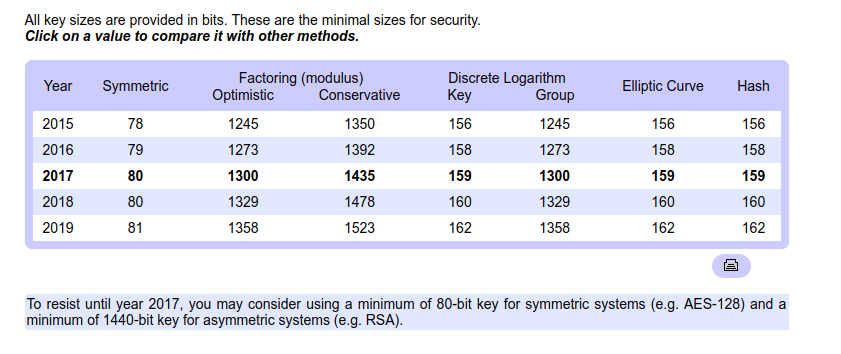
\includegraphics[width=120mm,scale=0.5]{keylengthcom.png}
  \end{figure}
\end{frame}

\begin{frame}{Impact on public-key cryptography}
\begin{itemize}
\item RSA: 4096
\item DH: 2048/256
\item Elliptic curve: 512/256 (bitcoin) 
\end{itemize}

NSA doesn't recommend elliptic curve cryptography for internal usage.
\end{frame}

%% \section{Заключение}
%% \begin{frame}{Что дальше?}
%% \begin{itemize}
%% \item Линейная алгебра (Матрицы)
%% \item Дискретная математика (Операции с остатком)
%% \end{itemize}
%% \end{frame}

\begin{frame}{Additional info}
https://github.com/ivanmurashko/lectures/tree/master/pdfs
 \begin{figure} 
   
\includegraphics[width=90mm,scale=0.5]{github.png}
  \end{figure}
\end{frame}

\begin{frame}{Questions}
 \begin{figure} 
   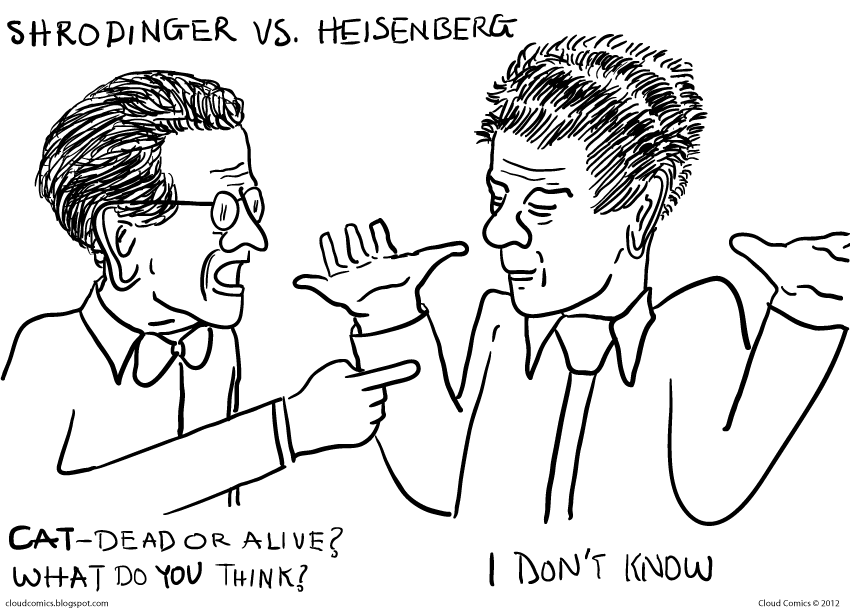
\includegraphics[width=90mm,scale=0.5]{questions.png}
  \end{figure}
\end{frame}

\end{document}
